\documentclass[addpoints]{exam}
\usepackage{preamble}
\sisetup{group-separator = {,}}

\pagestyle{headandfoot}
\runningheadrule


\firstpagefooter{Access for free at \href{https://openstax.org/books/astronomy-2e/pages/1-introduction}{https://openstax.org/books/astronomy-2e/pages/1-introduction}}{}{}
\runningfooter{Access for free at \href{https://openstax.org/books/astronomy-2e/pages/1-introduction}{https://openstax.org/books/astronomy-2e/pages/1-introduction}}{}{}


\firstpageheader{Astronomy}{Quiz}{Chapter 15: {\small The Sun (Part I)}}


\CorrectChoiceEmphasis{\color{red}\bfseries}
\SolutionEmphasis{\color{red}}
\printanswers

\begin{document}


\begin{questions}

% \begin{choices}
% \choice 
% \choice 
% \choice 
% \choice 
% \end{choices}

\question
Plasma \fillin\ .

\question
The photosphere \fillin\ .

\question
\fillin\ is known as the chromosphere.

\question
What is the corona?

\question
Solar wind is \fillin\ .

\question
\fillin\ is known as the aurora.

\question
What is a sunspot?

\question
What is a solar flare?

\question 
What is the most abundance element in the Sun?

\begin{choices}
\choice 
\correctchoice Hydrogen
\choice 
\choice 
\end{choices}

\question %predict, or higher level on Bloom's taxonomy
Which part of the Sun is visible during a total solar eclipse? (\textit{Warning}: Never look directly at the Sun.)
\vspace{1ex}

\begin{minipage}{0.3\textwidth}
    \centering
    \begin{choices}
    \choice 
    \choice 
    \correctchoice the corona 
    \choice 
    \end{choices}
\end{minipage}%
\begin{minipage}{0.5\textwidth}
    \centering
    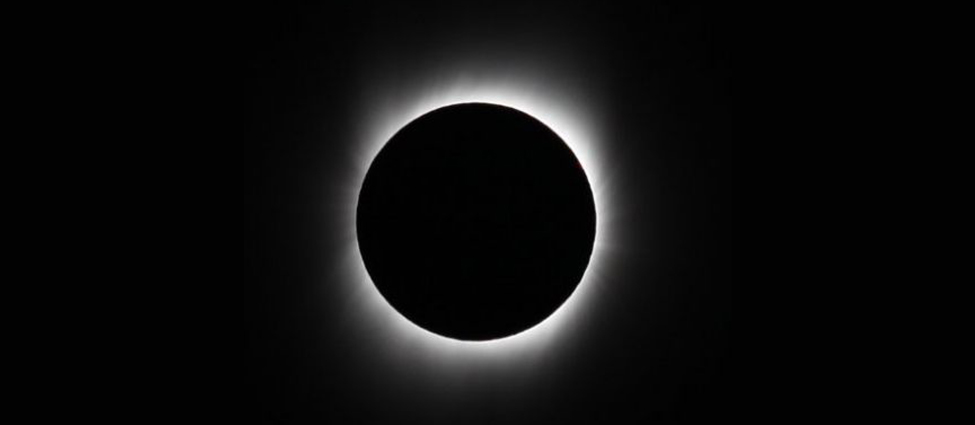
\includegraphics[width=0.5\textwidth,trim={1.5in 0 1.8in 0},clip]{Figures/Figure4.23.jpg}
    \captionof*{figure}{\small Credit: modification of work by Lutfar Rahman Nirjhar}
\end{minipage}
\vspace{1em}





\end{questions}
\end{document}